\documentclass[a4paper]{scrreprt}

\usepackage[ngerman]{babel}
\usepackage[utf8]{inputenc}
\usepackage[T1]{fontenc}
\usepackage{ae}
\usepackage[bookmarks, bookmarksnumbered]{hyperref}
\usepackage{tabularx}
\usepackage{graphicx}
\usepackage{csquotes}
\usepackage[nonumberlist, toc, section]{glossaries}
\usepackage[german]{fancyref}

\makeglossaries

\newglossaryentry{Produkt}
{
name=Produkt,
plural=Produkte,
description={Das von uns gelieferte Softwaresystem.}
}

\newglossaryentry{Webbrowser}
{
name=Webbrowser,
plural=Webbrowser,
description={Für dieses Produkt wird nur auf Google Chrome und Mozilla Firefox hin entwickelt.}
}

\newglossaryentry{Spiel}
{
name={Spiel},
plural={Spiele},
description={Ein Spiel ist eine Instanz eines \Gls{Spielmodus}. Ein Spiel hat das Ziel, das Wissen des Spielers zu nutzen, um die Merkmalsauswahl für Machine Learning zu unterstützen.}
}
\newglossaryentry{Spielmodus}
{
name={Spielmodus},
plural={Spielmodi},
description={Ein Spielmodus ist eine definierte Art und Weise, die Merkmalsauswahl durchzuführen. Standardmäßig gibt es die Spielmodi \Gls{Matrix Select} und \Gls{Binar Select}.}
}
\newglossaryentry{Matrix Select}
{
name={Matrix Select},
plural={Matrix Select},
description={Matrix Select ist ein \Gls{Spielmodus}, in dem ein \Gls{Spieler} aus einer bestimmten Anzahl an Merkmalen eine Teilmenge auswählt.}
}
\newglossaryentry{Binar Select}
{
name={Binär Select},
plural={Binär Select},
description={Binär Select ist ein \Gls{Spielmodus}, in dem ein \Gls{Spieler} Merkmale jeweils paarweise vergleicht und eins auswählt.}
}

\newglossaryentry{Spieler}
{
name=Spieler,
plural=Spieler,
description={Ein Nutzer, welcher an einem Spiel teilnimmt. Meist ist dies ein Angestellter des Betriebs.}
}

\newglossaryentry{Spieleinstellungen}
{
name=Spieleinstellungen,
plural=Spieleinstellungen,
description={Einstelllungen für ein Spiel umfassen: die Merkmale, welche ausgewählt werden soll, die Art des Spiels, die teilnehmenden Spieler, Endbedingungen des Spiels.}
}
\newglossaryentry{Organisator}
{
name=Organisator,
plural=Organisatoren,
description={Ein Organisator ist ein Nutzer, der neue Spiele erstellt und die Ergebnisse von diesen ausliest.}
}
\newglossaryentry{Achievement}
{
name=Achievement,
plural=Achievements,
description={Ein Ziel oder eine Errungenschaft, welche den Spieler motiviert, weiterzuspielen.}
}
\newglossaryentry{Administrator}
{
name=Administrator,
plural=Administratoren,
description={Die Person, welche das System installiert und den Nutzern zur Verfügung stellt. Sie verwaltet den
\Gls{Spiele-Server}}
}
\newglossaryentry{Spiele-Server}
{
name=Spiele-Server,
plural=Spiele-Server,
description={Ein Computer, welcher der Verwaltung von CS:Select dient und eine Internetanbindung hat.}
}

\begin{document}

    \title{Pflichtenheft CS-Select}
    \author{PSEArmee}
    \maketitle

    % Platzierung des Inhaltsverzeichnisses
    \tableofcontents

    \chapter{Zielbestimmung}
    Eine Organisation soll durch das \Gls{Produkt} das Domänenwissen ihrer Mitarbeiter dazu nutzen, die Merksmalsauswahl für ein Machine-Learning-Modell zu vereinfachen.

    \section{Musskriterien}
    \begin{tabular}{ l | l}
        /FA10/ & Ein \Gls{Spieler} muss sich anmelden können. \\
        /FA20/ & Ein \Gls{Spieler} muss sich registrieren können. \\
        /FA30/ & Ein \Gls{Organisator} muss sich anmelden können. \\
        /FA40/ & Ein \Gls{Organisator} muss ein \Gls{Spiel} erstellen und beenden können. \\
        /FA50/ & Die Anmeldung muss in einem modernem \Gls{Webbrowser} möglich sein. \\
        /FA60/ & \Gls{Spieler} müssen bei einem \Gls{Spiel} mitspielen können. \\
        /FA70/ & Ein \Gls{Organisator} muss \Gls{Spieler} zu einem \Gls{Spiel} einladen können. \\
        /FA80/ & Die Ergebnisse eines \Gls{Spiel} können ausgelesen werden. \\
        /FA90/ & Ein Spiel muss Endbedingungen besitzen. \\
        /FA100/ & Ein Spiel muss bei Erreichen seiner Endbedingungen enden. \\
        /FA110/ & Das System muss mit dem ML-Server kommunizieren. \\
        /FA120/ & Der Organisator kann in einem GUI den Spielstand überprüfen.\\
    \end{tabular}

    \section{Kannkriterien}
    \begin{tabularx}{\linewidth}{@{}>{\bfseries}l@{\hspace{.5em}}X@{}} % Linebreaks in der Tabelle
        /KA10/ & Ein \Gls{Organisator} kann die Ergebnisse/Eingabe eines Spielers ansehen. \\
        /KA20/ & Der \Gls{Administrator} kann Spiele aus dem System löschen. \\
        /KA30/ & Der \Gls{Organisator} kann Spiele löschen. \\
        /KA40/ & Ein \Gls{Organisator} kann eines seiner \Glspl{Spiel} löschen. \\
        /KA50/ & Der \Gls{Spiele-Server} kann vom Terminal aus beendet werden. \\
        /KA60/ & Beim Erstellen eines Spiels kann der \Gls{Organisator} die \Gls{Spieleinstellungen} speichern und laden. \\
        /KA70/ & Das System kann auf verschiedenen Ports ausgeführt werden. \\
        /KA80/ & Beim Start des Systems erscheint ein Dialog zum Einrichten des Systems. \\
        /KA90/ & Die Ergebnisse eines \Gls{Spiel}s werden im Interface des \Gls{Organisator}s angezeigt. \\
        /KA100/ & Beim Spielen existiert ein Knopf, welcher das Überspringen der aktuellen Runde ermöglicht. \\
        /KA110/ & Der Knopf aus /KA100/ kostet den \Gls{Spieler} Punkte beim Betätigen. \\
        /KA120/ & Es ist \Gls{Spieler}n möglich Kriterien auszuschließen, also diese als unwichtig zu markieren. \\
        /KA130/ & Der \Gls{Organisator} eines Spiels kann nach dem Begin eines Spiels noch weitere Spieler einladen. \\
        /KA140/ & Die Merkmale, die pro Runde angezeigt werden, sind schlauer ausgewählt als durch Zufall. \\ %Schlauer präzisieren? Da mir nichts einfällt kann ich da wenig präzisieren
        /KA150/ & Die maximale Anzahl an Runden pro Spieler pro Tag können durch den \Gls{Organisator} eingeschränkt werden. \\
        /KA160/ & \Glspl{Spieler} erhalten mehr Punkte, wenn sie mehrere Runden in Folge spielen. \\
        /KA170/ & Es gibt \Gls{Achievement}s, welche von Spielern freigeschaltet werden. \\
        /KA180/ & Es gibt eine Auflistung der \Gls{Achievement}s aus /KA170/. \\
        /KA190/ & Es gibt eine Hilfe Schaltfläche im \Gls{Spieler} GUI. \\ 
        /KA200/ & Es gibt eine Hilfe Schaltfläche im \Gls{Organisator} GUI. \\ 
        /KA210/ & Das Webinterface unterstüzt Internet Explorer. \\
        /KA220/ & Mehrere Sprachen sind einfach zu integrieren. \\
        /KA230/ & Es ist möglich die Punkte eines \Gls{Spieler}s zurückzusetzten. \\ %Durch Spieler oder Orga?
        /KA240/ & Es gibt eine GUI für \Glspl{Administrator}. \\ 
    \end{tabularx}

    \section{Abgrenzungskriterien}
    \begin{tabular}{ l | l}
    /AK10/ & Das Produkt muss nicht bestimmen welches Subset an Merkmalen optimal ist.\\
    /AK20/ & Das Produkt muss nicht die Auswertung der Ergebnisse unterstützen.\\
    /AK30/ & \\
    /AK40/ & \\
    /AK50/ & \\
    /AK60/ & \\
    /AK70/ & \\
    /AK80/ & \\
    /AK90/ & \\
    /AK100/ & \\
    /AK110/ & \\
    /AK120/ & \\
    /AK130/ & \\
    \end{tabular}

    \chapter{Einsatz}

    \section{Anwendungsbereiche}
    Das \Gls{Produkt} dient der Verbesserung der Merkmalsauswahl bei Machine-Learning Prozessen in wissenschaftlichen
    Experimenten beziehungsweise privatwirtschaftlichen Unternehmen durch das Domänenwissen der \Gls{Spieler}.

    \section{Zielgruppen}
    Die Zielgruppen des \Gls{Produkt}s lassen sich in \Glspl{Organisator} und \Glspl{Spieler} unterscheiden.
    Der Organisator möchte eine Verbesserung der Machine-Learning Prozesse erreichen indem er das Domänenwissen der Spieler nutzt.
    Die Spieler tragen durch Spielen des \Gls{Produkt}s mit ihrem Domänenwissen zur besseren Merkmalsauswahl bei.

    \section{Betriebsbedingungen}
    Das \Gls{Produkt} ist für die Nutzung in Büroräumlichkeiten vorgesehen.

    \chapter{Umgebung}
    Das \Gls{Produkt} läuft auf einem Server, die Nutzung erfolgt an Arbeitsplatzrechnern.

    \section{Software}
    Das \Gls{Produkt} läuft auf Linux ab Kernel Version 4 und Windows 7 oder neuer.

    \section{Hardware}
    Das \Gls{Produkt} läuft auf Server-Computern.

    \chapter{Produktdaten}

    \section{Nutzerdaten}
    \begin{tabularx}{\linewidth}{@{}>{\bfseries}l@{\hspace{.5em}}X@{}}
        /D10/ & Über Nutzer(\Gls{Spieler}, \Gls{Organisator}) sind folgende Daten zu speichern /ND10/: 
        \begin{itemize}
              \item Email-Adresse, Nutzername, Punktestand, Rolle, Passwort(als Hash)
        \end{itemize} \\
        /KD10/ & Über einen \Gls{Spieler} werden außerdem seine Achievements gespeichert. \\
        /KD20/ & Über einen \Gls{Organisator} werden außerdem seine Spieleinstellungen gespeichert. \\
    \end{tabularx}

    \section{Merkmalsdatensätze}
    \begin{tabularx}{\linewidth}{@{}>{\bfseries}l@{\hspace{.5em}}X@{}}
        /D20/ & Für jeden Merkmalsdatensatz ist zu speichern: /ND20/: 
        \begin{itemize}
             \item Liste an Merkmalen mit jeweiligen Graphen und Beschreibung
        \end{itemize}
    \end{tabularx}

    \section{Spieledaten}
    \begin{tabularx}{\linewidth}{@{}>{\bfseries}l@{\hspace{.5em}}X@{}}
        /D30/ & Für jedes \Gls{Spiel} ist zu speichern /ND30/: 
        \begin{itemize}
             \item \Gls{Organisator}, \Gls{Spieleinstellungen}, \Gls{Spieler}, zugehöriger Merkmalsdatensatz % zuständiger ML Server?
        \end{itemize}
    \end{tabularx}


    \chapter{Nichtfunktionale Anforderungen}

    \begin{tabular}{ l | l}
        /NF10/ & Es müssen mindestens 30 Spieler zur gleichen Zeit spielen können.\\
        /NF20/ & Die Interaktionszeiten dürfen nicht länger als zwei Sekunden betragen. \\
        /NF30/ & Ein Spieler soll das Ergebnis eines Spiels innerhalb von zwei Sekunden erhalten. \\
        /NF40/ & Das Design soll modern sein. \\
        /NF50/ & Die ML-Datenbanken sollen leicht austauschbar sein. \\
        /NF60/ & Neue Spielmodi sollen leicht erweitert werden können. \\
        /NF70/ & Neue Sprachen sollen leicht hinzugefügt werden können. \\
        /NF80/ & Das Produkt enthält nicht mehr als 0,1\% plattformspezifischer Anweisungen. \\
        /NF90/ & Es gibt nicht mehr als einen Ausfall des Systems pro Monat. \\ %Realistisch?
        /NF100/ & \\
        /NF110/ & \\
        /NF120/ & \\
    \end{tabular}

    \chapter{Systemmodelle}

    \section{Szenarien}
    \newpage

    \section{Anwendungsfälle}

    \subsection{Ergebnisse auslesen}
    \begin{itemize}
        \item Teilnehmende Akteure: \Gls{Organisator}
        \item Eingangsaktionen: \Gls{Organisator} öffnet die Auswertungsseite
        \item Ausgangsaktionen: \Gls{Organisator} erhält die Auswertung
        \item Ereignisfluss -
    \end{itemize}

    \subsection{Server installieren}
    \begin{itemize}
        \item Teilnehmende Akteure: \Gls{Administrator} 
        \item Eingangsaktionen: Computer mit MySQL und Tomcat installiert
        \item Ausgangsaktionen: Spiele-Server starten
        \item Ereignisfluss: 
            \begin{itemize}
                \item Administrator kopiert die War datei in den Tomcat webapps Ordner
                \item Administrator fügt den Pfad zur CFG Datei in die `tomcat/conf/Catalina/<host>` Datei ein
                \item Administrator konfiguriert die CFG Datei aus der Dokumentation mit den relevanten Werten
                \item Administrator führt \texttt{tomcat/bin/startup.sh}(Linux \& Mac) bzw. \texttt{tomcat\textbackslash bin\textbackslash startup.bat}(Windows) aus
            \end{itemize}
    \end{itemize}

    \subsection{Server beenden}
    \begin{itemize}
        \item Teilnehmende Akteure: Administrator
        \item Eingangsaktionen: Spiele-Server ist aktiv
        \item Ausgangsaktion: MySQL beenden, falls sonst nichts Weiteres auf der Datenbank läuft
        \item Ereignisfluss: Administrator führt \texttt{tomcat/bin/shutdown.sh}(Linux \& Mac) bzw. \texttt{tomcat\textbackslash bin\textbackslash shutdown.bat}(Windows)
    \end{itemize}

    \subsection{Spieler registrieren}
    \begin{itemize}
        \item Teilnehmende Akteure: Organisator, Spieler
        \item Eingangsaktionen: Spiele-Server ist aktiv
        \item Ereignisfluss:
        \begin{itemize}
            \item Organisator lädt den Spieler über das Organisator-GUI ein.
            \item Der Spieler klickt auf den Einladungslink in der E-Mail und wird auf die Registrierungsseite weitergeleitet.
            \item Der Spieler gibt einen einzigartigen Nutzernamen, seine E-Mail-Addresse sowie ein persönliches Passwort ein und bestätigt.
        \end{itemize}
    \end{itemize}

    \subsection{Spieler anmelden}
    \begin{itemize}
        \item Teilnehmende Akteure: Spieler
        \item Eingangsaktionen: Spiele-Server ist aktiv
        \item Ereignisfluss:
        \begin{itemize}
            \item Spieler öffnet die Produktwebsite
            \item Spieler wählt die Rolle "Spieler" aus
            \item Spieler gibt E-Mail und Passwort ein
            \item Spieler klickt auf anmelden
        \end{itemize}
    \end{itemize}

    \subsection{Spieler löschen}
    \begin{itemize}
        \item Teilnehmende Akteure: Administrator
        \item Eingangsaktionen: Spiele-Server ist aktiv
        \item Ereignisfluss:
        \begin{itemize}
            \item Administrator loggt sich am Server ein
            \item Administrator führt das Löschen-Kommando mit dem Nutzernamen des zu löschenden Spielers aus
            \item Administrator bestätigt den Vorgang
        \end{itemize}
    \end{itemize}

    \subsection{Organisator registrieren}
    \begin{itemize}
        \item Teilnehmende Akteure: Organisator
        \item Eingangsaktionen: Spiele-Server ist aktiv, Organisator-Registrierungspasswort ist gesetzt.
        \item Ereignisfluss:
        \begin{itemize}
            \item Der Organisator öffnet die Produktwebsite und klickt auf Registrieren.
            \item Der Spieler gibt einen einzigartigen Nutzernamen, seine E-Mail-Addresse, das Organisator-Registrierungspasswort sowie ein persönliches Passwort ein und bestätigt.
        \end{itemize}
    \end{itemize}

    \subsection{Organisator anmelden}
    \begin{itemize}
        \item Teilnehmende Akteure: Organisator
        \item Eingangsaktionen: Spiele-Server ist aktiv
        \item Ereignisfluss:
        \begin{itemize}
            \item Organisator öffnet die Produktwebsite
            \item Organisator wählt die Rolle "Organisator" aus
            \item Organisator gibt E-Mail und Passwort ein
            \item Organisator klickt auf anmelden
        \end{itemize}
    \end{itemize}

    \subsection{Organisator löschen}
    \begin{itemize}
        \item Teilnehmende Akteure: Administrator
        \item Eingangsaktionen: Spiele-Server ist aktiv
        \item Ereignisfluss:
        \begin{itemize}
            \item Administrator loggt sich am Server ein
            \item Administrator führt das Löschen-Kommando mit dem Nutzernamen des zu löschenden Organisators aus
            \item Administrator bestätigt den Vorgang
        \end{itemize}
    \end{itemize}

    \subsection{Spiel erstellen}
    \begin{itemize}
        \item Teilnehmende Akteure: \Gls{Organisator}
        \item Eingangsaktionen: Spiele-Server ist aktiv
        \item Ausgangsaktionen: Spiel starten
        \item Ereignisfluss:
        \begin{itemize}
            \item Organisator meldet sich an
            \item Organisator sucht sich über seine GUI die gewünschten Spieleinstellungen aus
            \item Organisator bestätigt seine Auswahl und erstellt das Spiel
        \end{itemize}
    \end{itemize}

    \subsection{Spiel löschen}
    \begin{itemize}
        \item Teilnehmende Akteure: \Gls{Organisator}
        \item Eingangsaktionen: Spiele-Server ist aktiv, es existiert bereits ein Spiel
        \item Ausgangsaktionen: Spiel löschen
        \item Ereignisfluss:
        \begin{itemize}
            \item Organisator meldet sich an
            \item Organisator wählt über seine GUI das zu löschende Spiel
            \item Organisator bestätigt seine Auswahl
        \end{itemize}
    \end{itemize}

    \subsection{Spieleinstellungen speichern}
    \begin{itemize}
        \item Teilnehmende Akteure: \Gls{Organisator}
        \item Eingangsaktionen: Spiele-Server ist aktiv
        \item Ausgangsaktionen: Spieleinstellungen wiederverwenden
        \item Ereignisfluss:
        \begin{itemize}
            \item Organisator meldet sich an
            \item Organisator sucht sich über seine GUI das Spiel aus, von dem er die Einstellungen speichern möchte
            \item Organisator wählt die Option \enquote{Spieleinstellungen speichern}
            \item Organisator bestätigt seine Auswahl und speichert die Einstellungen
        \end{itemize}
    \end{itemize}

    \subsection{Spieleinstellungen laden}
    \begin{itemize}
        \item Teilnehmende Akteure: \Gls{Organisator}
        \item Eingangsaktionen: Spiele-Server ist aktiv, Spieleinstellungen wurden bereits gespeichert
        \item Ausgangsaktionen: Spiel starten
        \item Ereignisfluss:
        \begin{itemize}
            \item Organisator meldet sich an
            \item Organisator erstellt über seine GUI ein neues Spiel
            \item Organisator wählt für dieses Spiel \enquote{Spieleinstellungen laden}
            \item Organisator sucht sich die bereits gespeicherte Spieleinstellungen heraus
            \item Organisator bestätigt seine Auswahl
        \end{itemize}
    \end{itemize}

    \subsection{Admin-Account einrichten}
    \begin{itemize}
        \item Teilnehmende Akteure: \Gls{Administrator}
        \item Eingangsaktionen: %??
        \item Ausgangsaktionen: Admin-Account erstellen
        \item Ereignisfluss:
        \begin{itemize}
            \item Admin-Account wird in einer config-Datei festgelegt
            \item Man gibt Name, E-Mail und Passwort des Admins ein
        \end{itemize}
    \end{itemize}
    %Beim erstmaligen Aufsetzen des \Gls{Spiele-Server}s kann ein Admin-Account in einer config-Datei festgelegt werden.
    %Dazu werden Name, Email und Passwort des \Gls{Administrator}s gespeichert.

    \subsection{Achievements ansehen}
    \begin{itemize}
        \item Teilnehmende Akteure: \Gls{Spieler}
        \item Eingangsaktionen: Spiele-Server ist aktiv
        \item Ausgangsaktionen: Achievements ansehen
        \item Ereignisfluss:
        \begin{itemize}
            \item Spieler meldet sich an
            \item Spieler erreicht seine Übersichts-Seite
            \item Spieler klickt auf die Spieler-Übersichts-Schaltfläche
            \item Spieler schaut seine Achievements an
        \end{itemize}
    \end{itemize}
    %Nach der Anmeldung erreicht ein \Gls{Spieler} eine Übersichts-Seite. Beim Klicken auf die Spieler-Übersicht-Schaltfläche
    %(in \fref{fig:Spieler-Übersicht} gezeigt) kann der \Gls{Spieler} seine \Gls{Achievement}s einsehen.

    \subsection{Leaderboard ansehen}
    \begin{itemize}
        \item Teilnehmende Akteure: \Gls{Spieler}
        \item Eingangsaktionen: Spiele-Server ist aktiv
        \item Ausgangsaktionen: Leaderboard ansehen
        \item Ereignisfluss:
        \begin{itemize}
            \item Spieler meldet sich an
            \item Spieler erreicht seine Übersichtsseite
            \item Spieler sieht dort in einer Tabelle die Spieler mit den meisten Punkten über einen gewissen Zeitraum
        \end{itemize}
    \end{itemize}
    %Nach der Anmeldung erreicht ein \Gls{Spieler} eine Übersichts-Seite. Darauf ist ein Bereich, der eine aktuelle Tabelle
    %anzeigt, in welcher die \Gls{Spieler} aufgelistet sind, die in einem bestimmten Zeitraum die meisten Punkte erreicht haben.
    
    \subsection{Runde spielen Matrix Select}
    \begin{itemize}
    	\item Teilnehmende Akteure: \Gls{Spieler}
    	\item Eingangsaktionen: Spiele-Server ist aktiv, Spieler hat offenes Spiel des Spielmodus Matrix Select
    	\item Ereignisfluss:
    	\begin{itemize}
    		\item Spieler meldet sich an
    		\item Spieler erreicht seine Übersichtsseite
    		\item Spieler klickt auf Weiterspielen-Schaltfläche
    		\item Spieler erreicht Spiel-GUI
    		\item Spieler klickt auf ein Merkmal und sieht Merkmalsgraphen und Merkmalsbeschreibung
    		\item Spieler wählt mehrere Merkmale aus
    		\item Spieler klickt auf Schaltfläche, um Auswahl zu bestätigen 
    	\end{itemize}
    \end{itemize}
	
	\subsection{Runde spielen Binär Select}
	\begin{itemize}
		\item Teilnehmende Akteure: \Gls{Spieler}
		\item Eingangsaktionen: Spiele-Server ist aktiv, Spieler hat offenes Spiel des Spielmodus Binär Select
		\item Ereignisfluss:
		\begin{itemize}
			\item Spieler meldet sich an
			\item Spieler erreicht seine Übersichtsseite
			\item Spieler klickt auf Weiterspielen-Schaltfläche
			\item Spieler erreicht Spiel-GUI
			\item Spieler klickt auf ein Merkmal und sieht Merkmalsgraphen und Merkmalsbeschreibung
			\item Spieler wählt eines der beiden Merkmale aus
			\item Spieler klickt auf Schaltfläche, um Auswahl zu bestätigen 
		\end{itemize}
	\end{itemize}

	\subsection{Runde überspringen}
	\begin{itemize}
		\item Teilnehmende Akteure: \Gls{Spieler}
		\item Eingangsaktionen: Spiele-Server ist aktiv, Spieler hat offenes Spiel 
		\item Ereignisfluss:
		\begin{itemize}
			\item Spieler meldet sich an
			\item Spieler erreicht seine Übersichtsseite
			\item Spieler klickt auf Weiterspielen-Schaltfläche
			\item Spieler erreicht Spiel-GUI
			\item Spieler klickt Runde-Überspringen-Schaltfläche und bestätigt seine Auswahl
		\end{itemize}
	\end{itemize}

	\subsection{Spielzustand auslesen}
	\begin{itemize}
		\item Teilnehmende Akteure: \Gls{Organisator}
		\item Eingangsaktionen: Spiele-Server ist aktiv
		\item Ereignisfluss:
		\begin{itemize}
			\item Organisator meldet sich an
			\item Organisator erreicht seine Übersichtsseite
			\item Organisator sieht den Zustand seiner laufenden Spiele
		\end{itemize}
	\end{itemize}

    \section{Objektmodell}

    \section{Dynamische Modelle}

    \section{Benutzerschnittstelle}

    \subsection{Anmeldung}
    \centering
    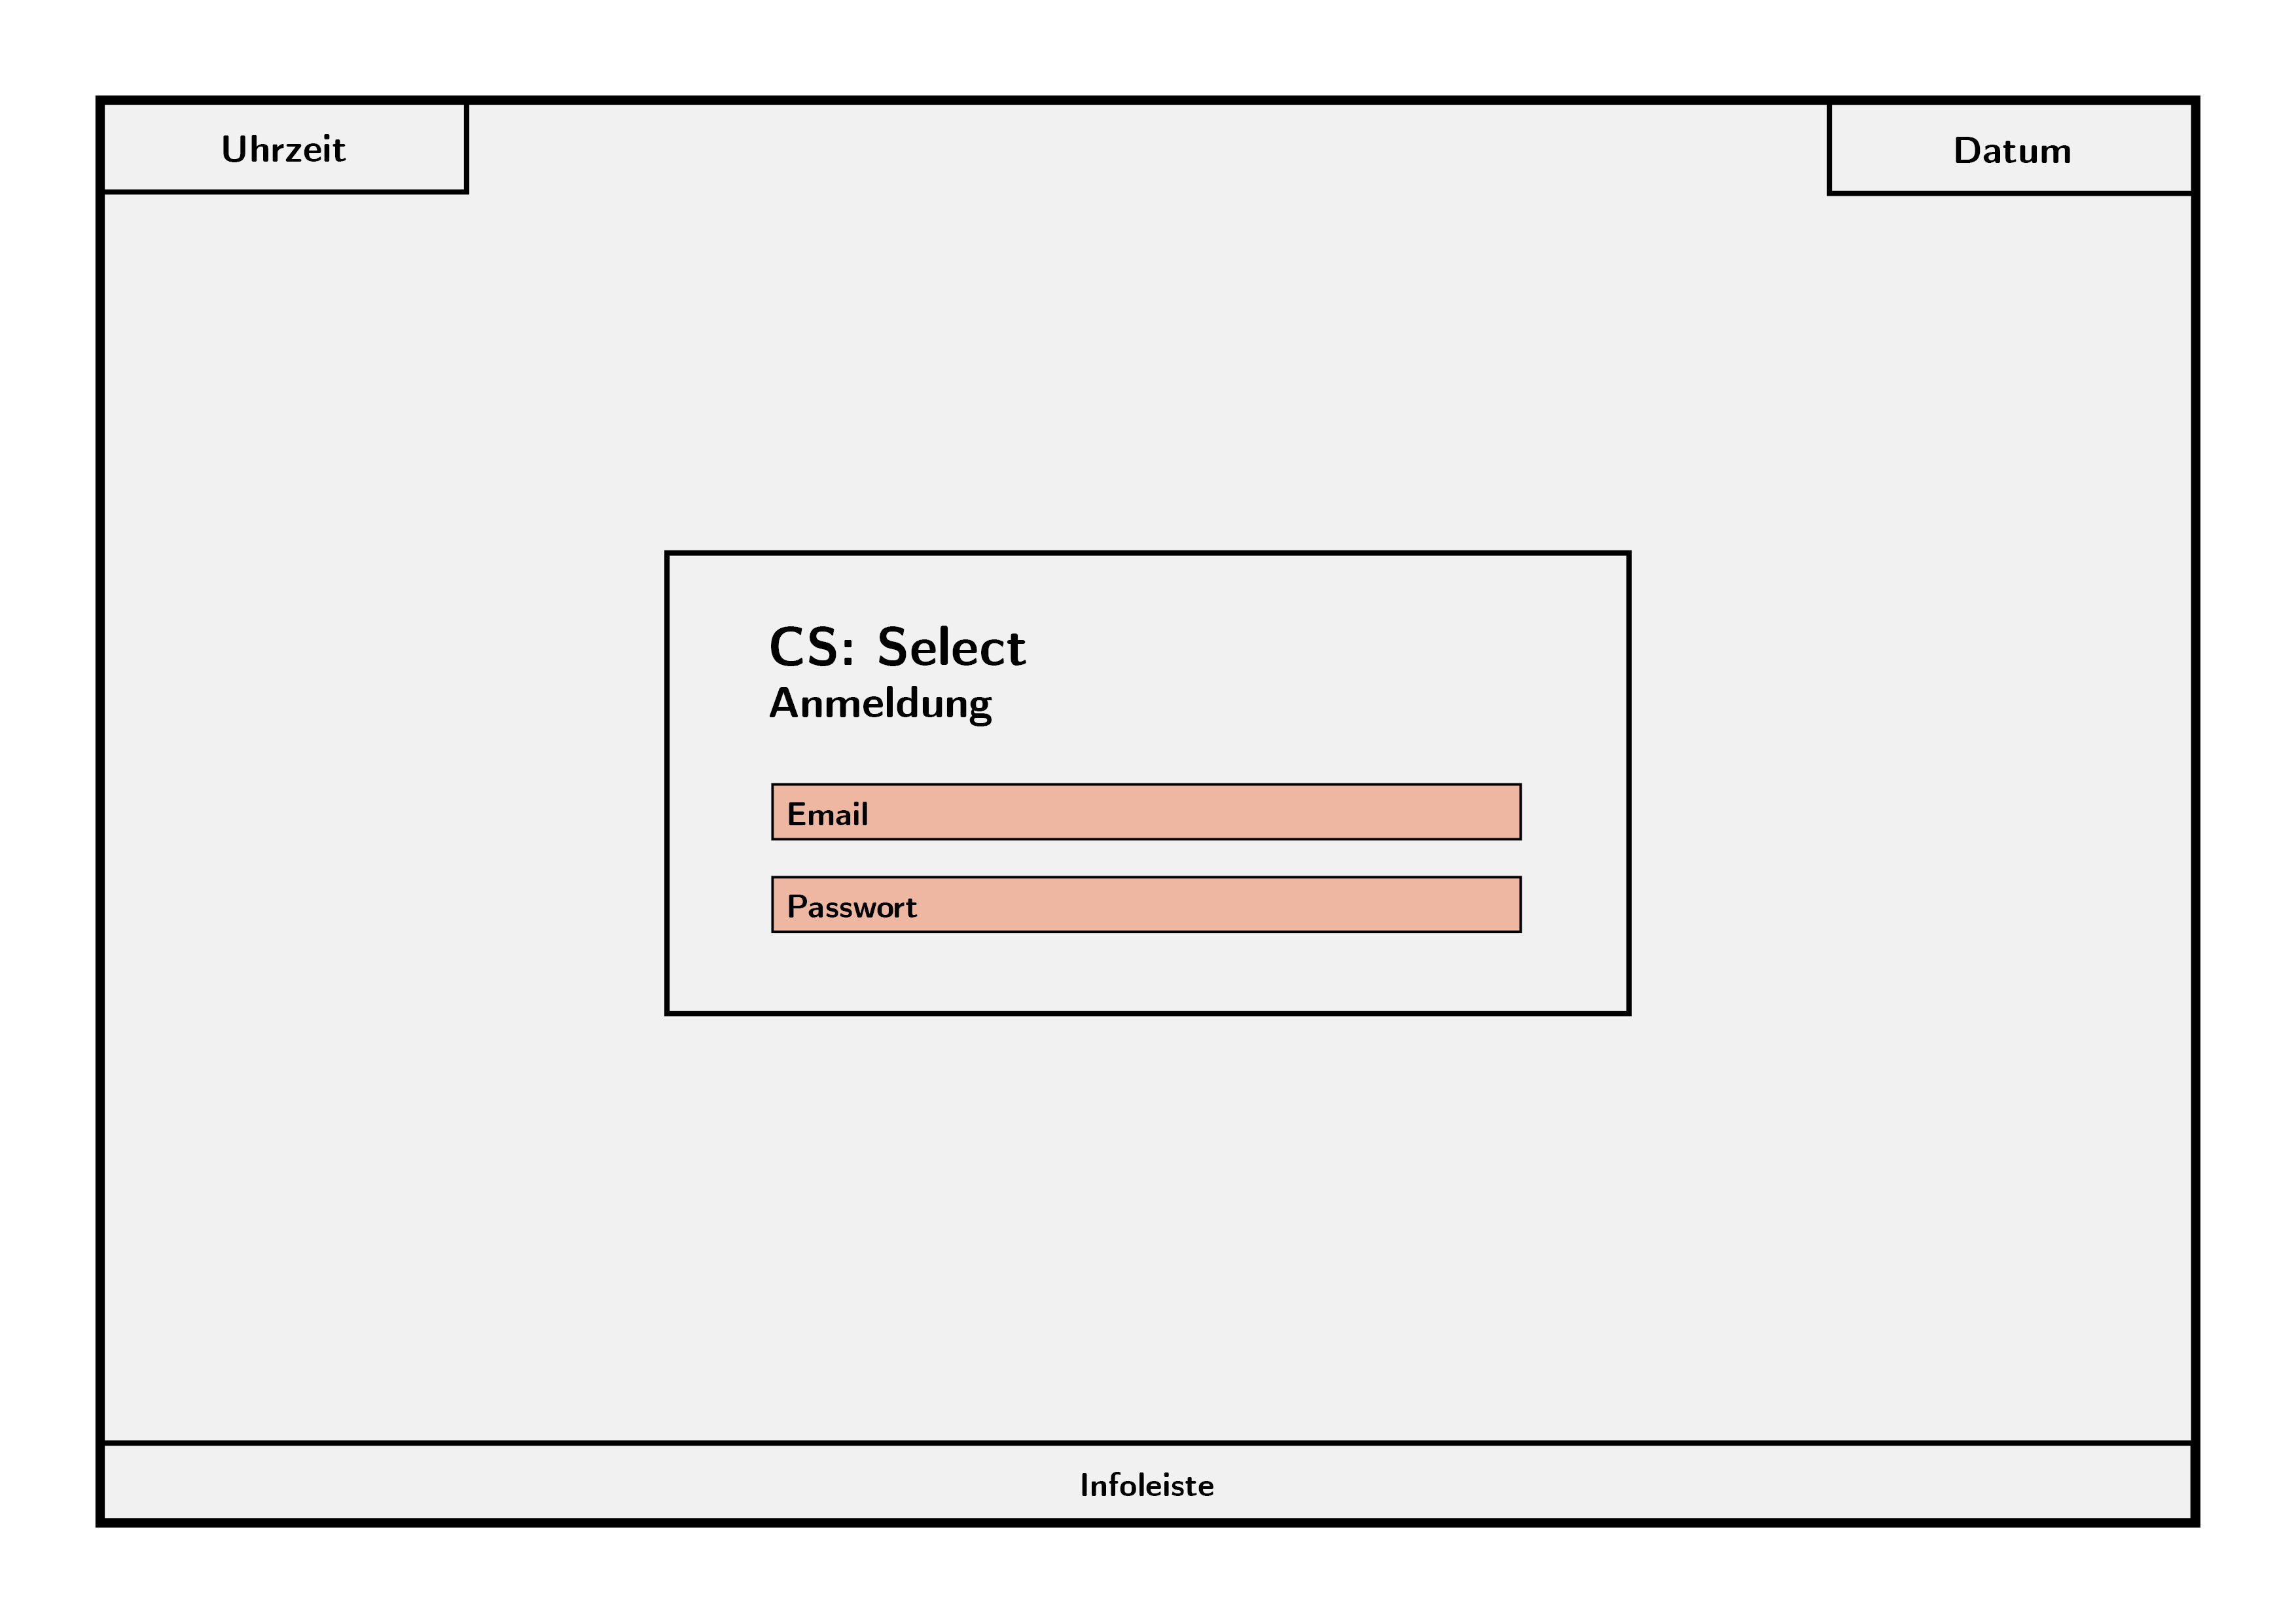
\includegraphics[width=400px]{../pictures/1_Anmeldung.jpg}
    %\caption{Anmeldung} %Nur ein Test

    \subsection{Organisator-Start (Desktop)}
    \centering
    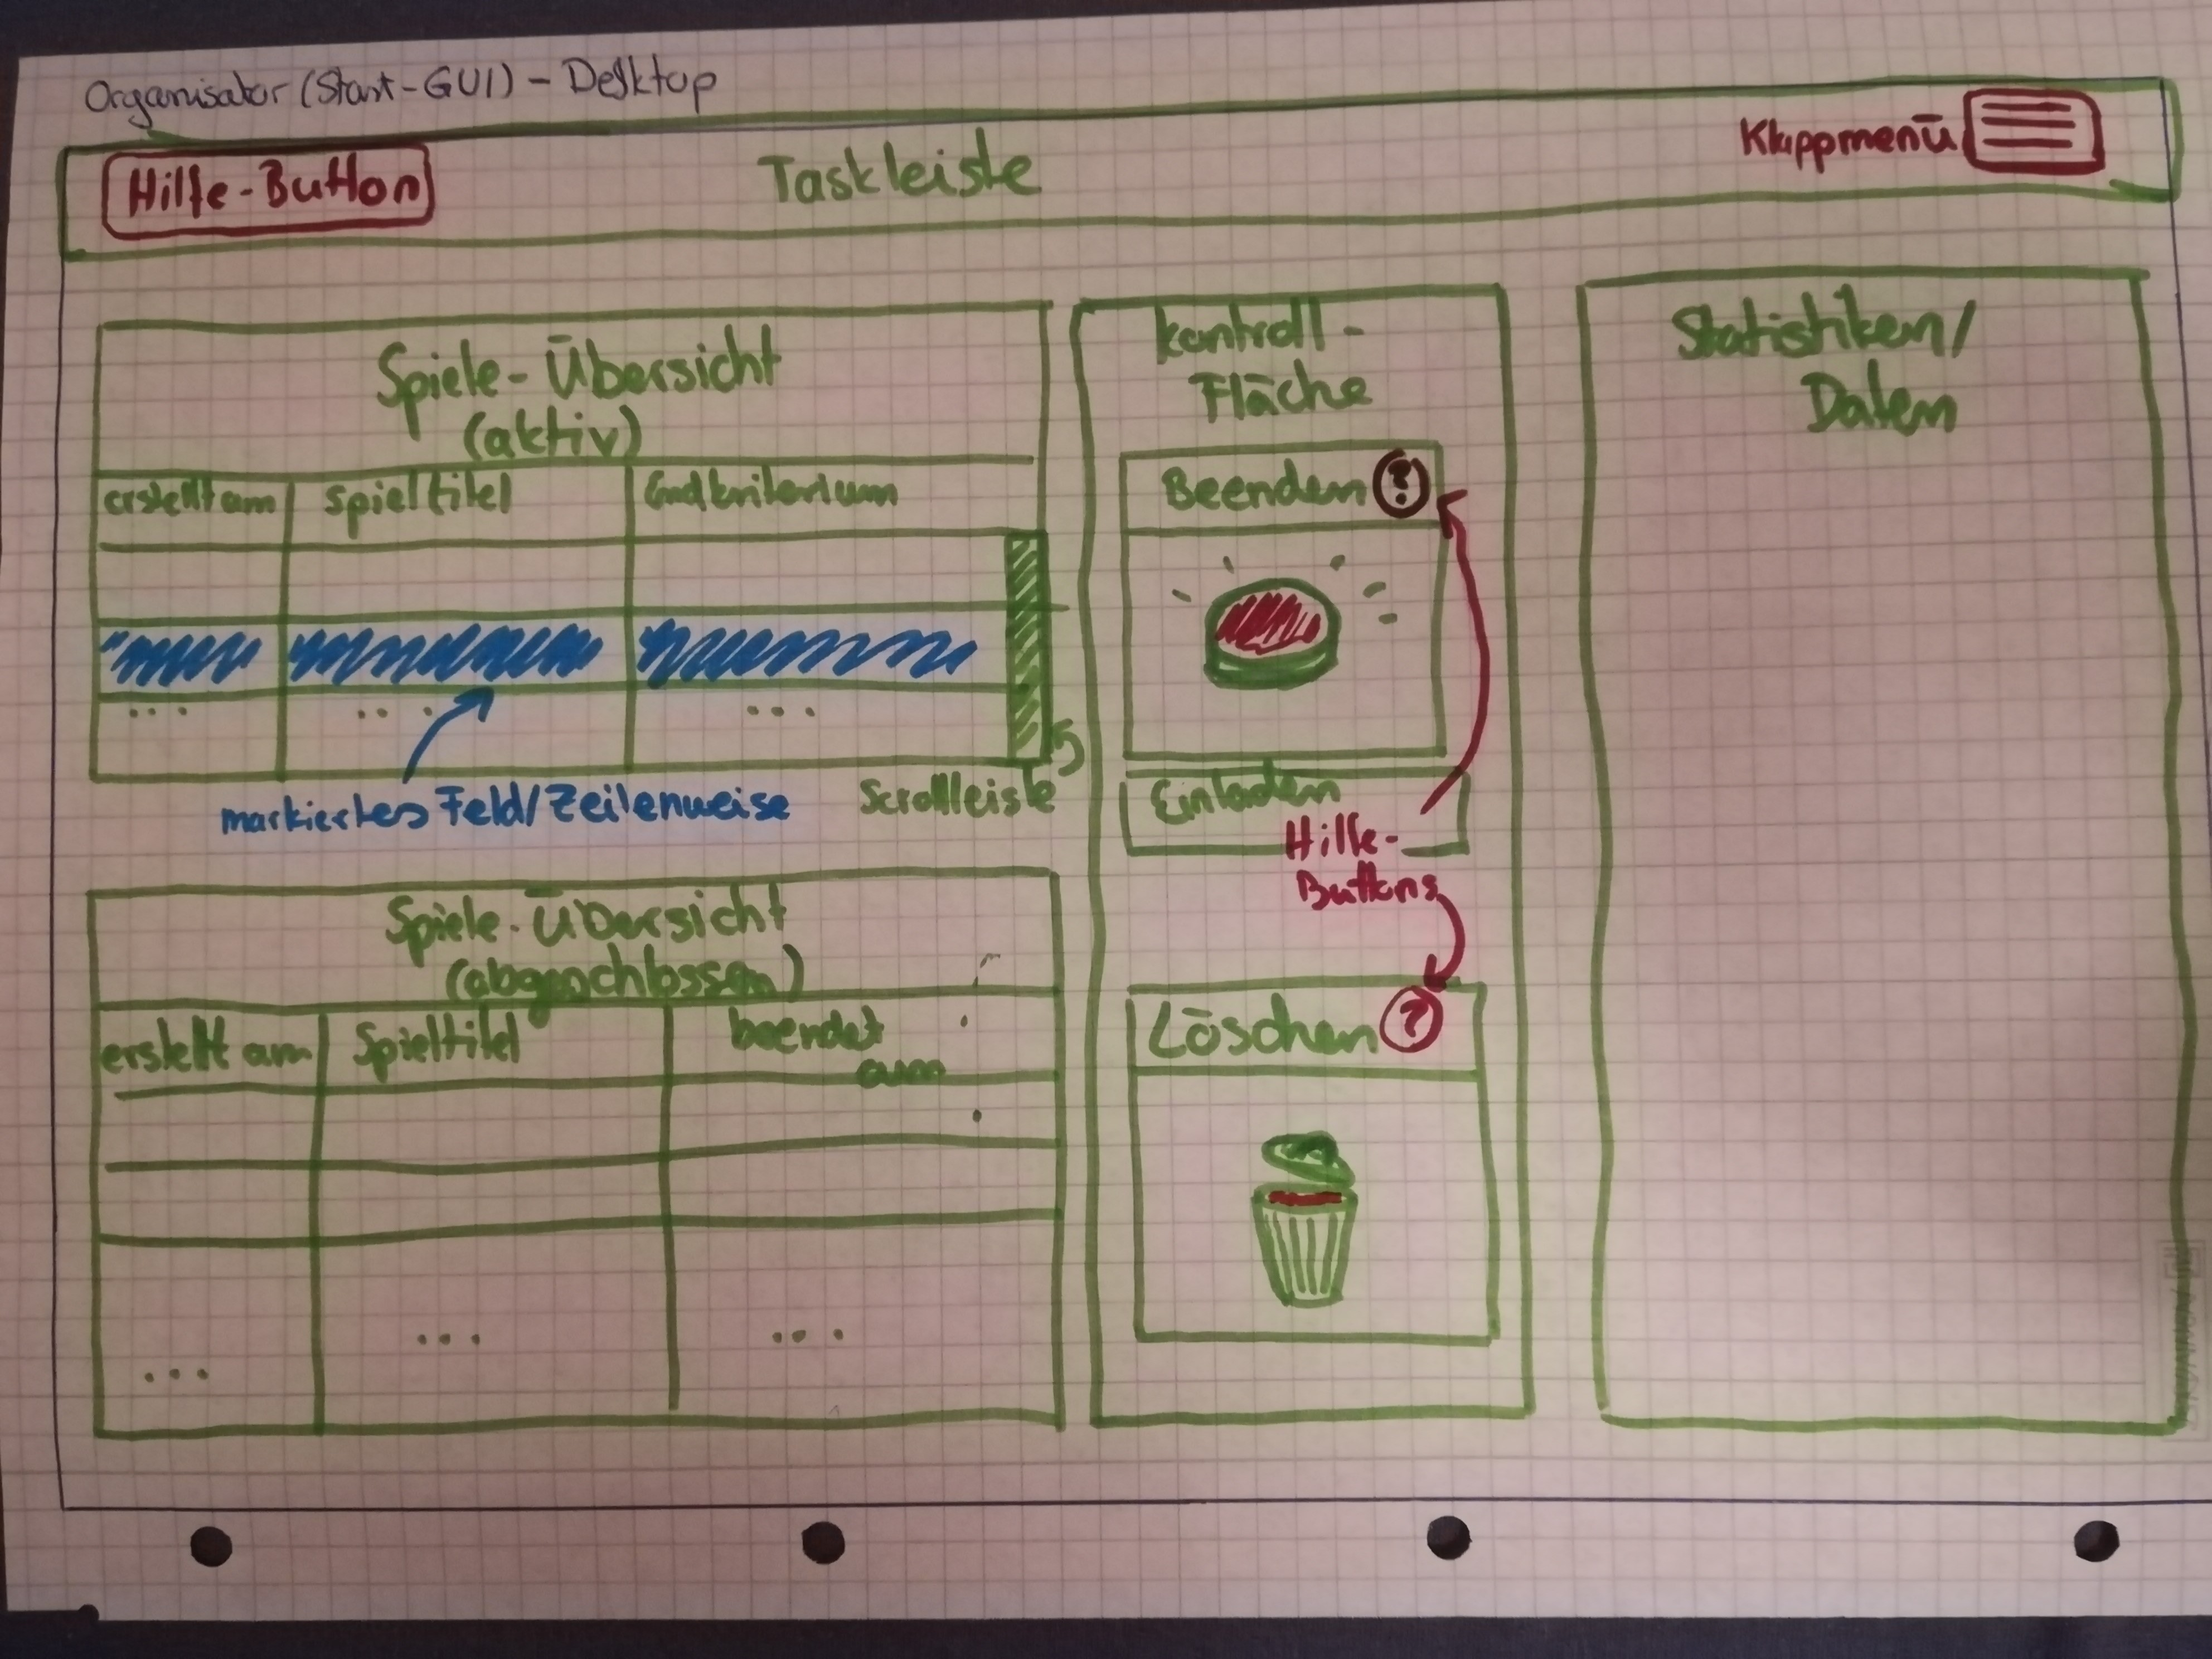
\includegraphics[width=400px]{../pictures/2_Organisator.jpg}

    \subsection{Organisator-Start (Responsive)}
    \centering
    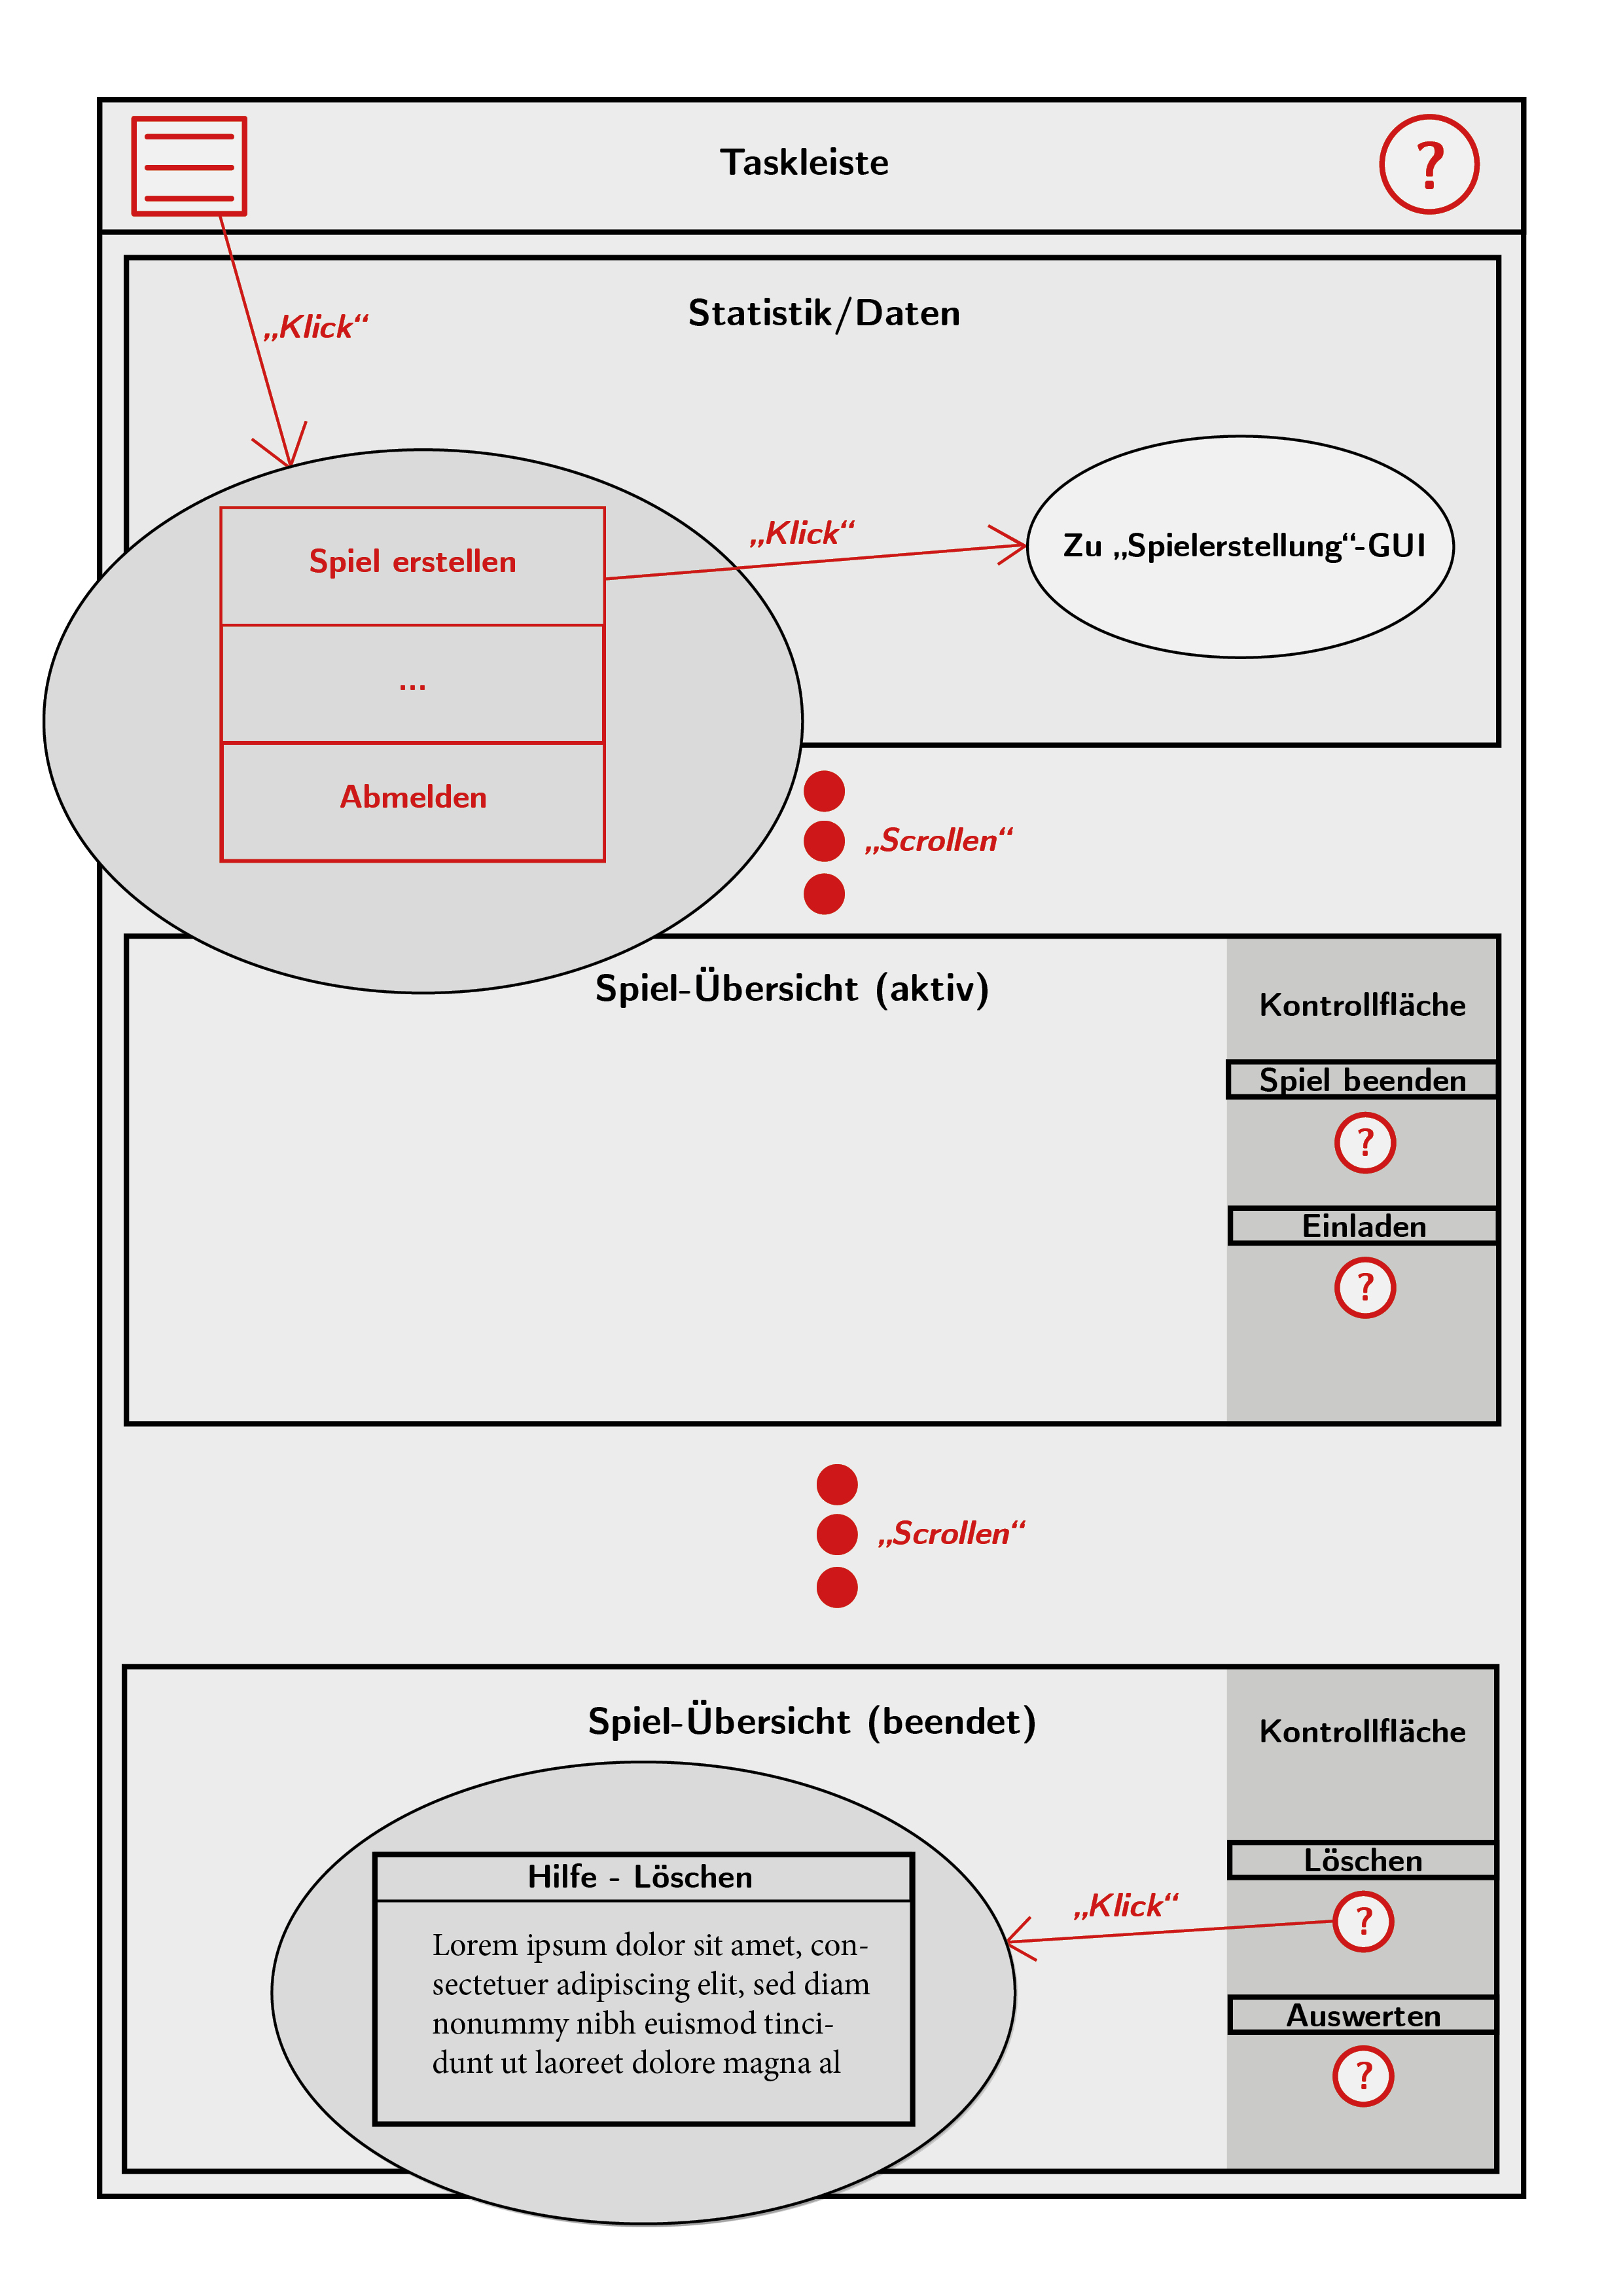
\includegraphics[width=400px]{../pictures/3_Organisator(responsive).jpg}

    \subsection{Spielerstellung}
    \centering
    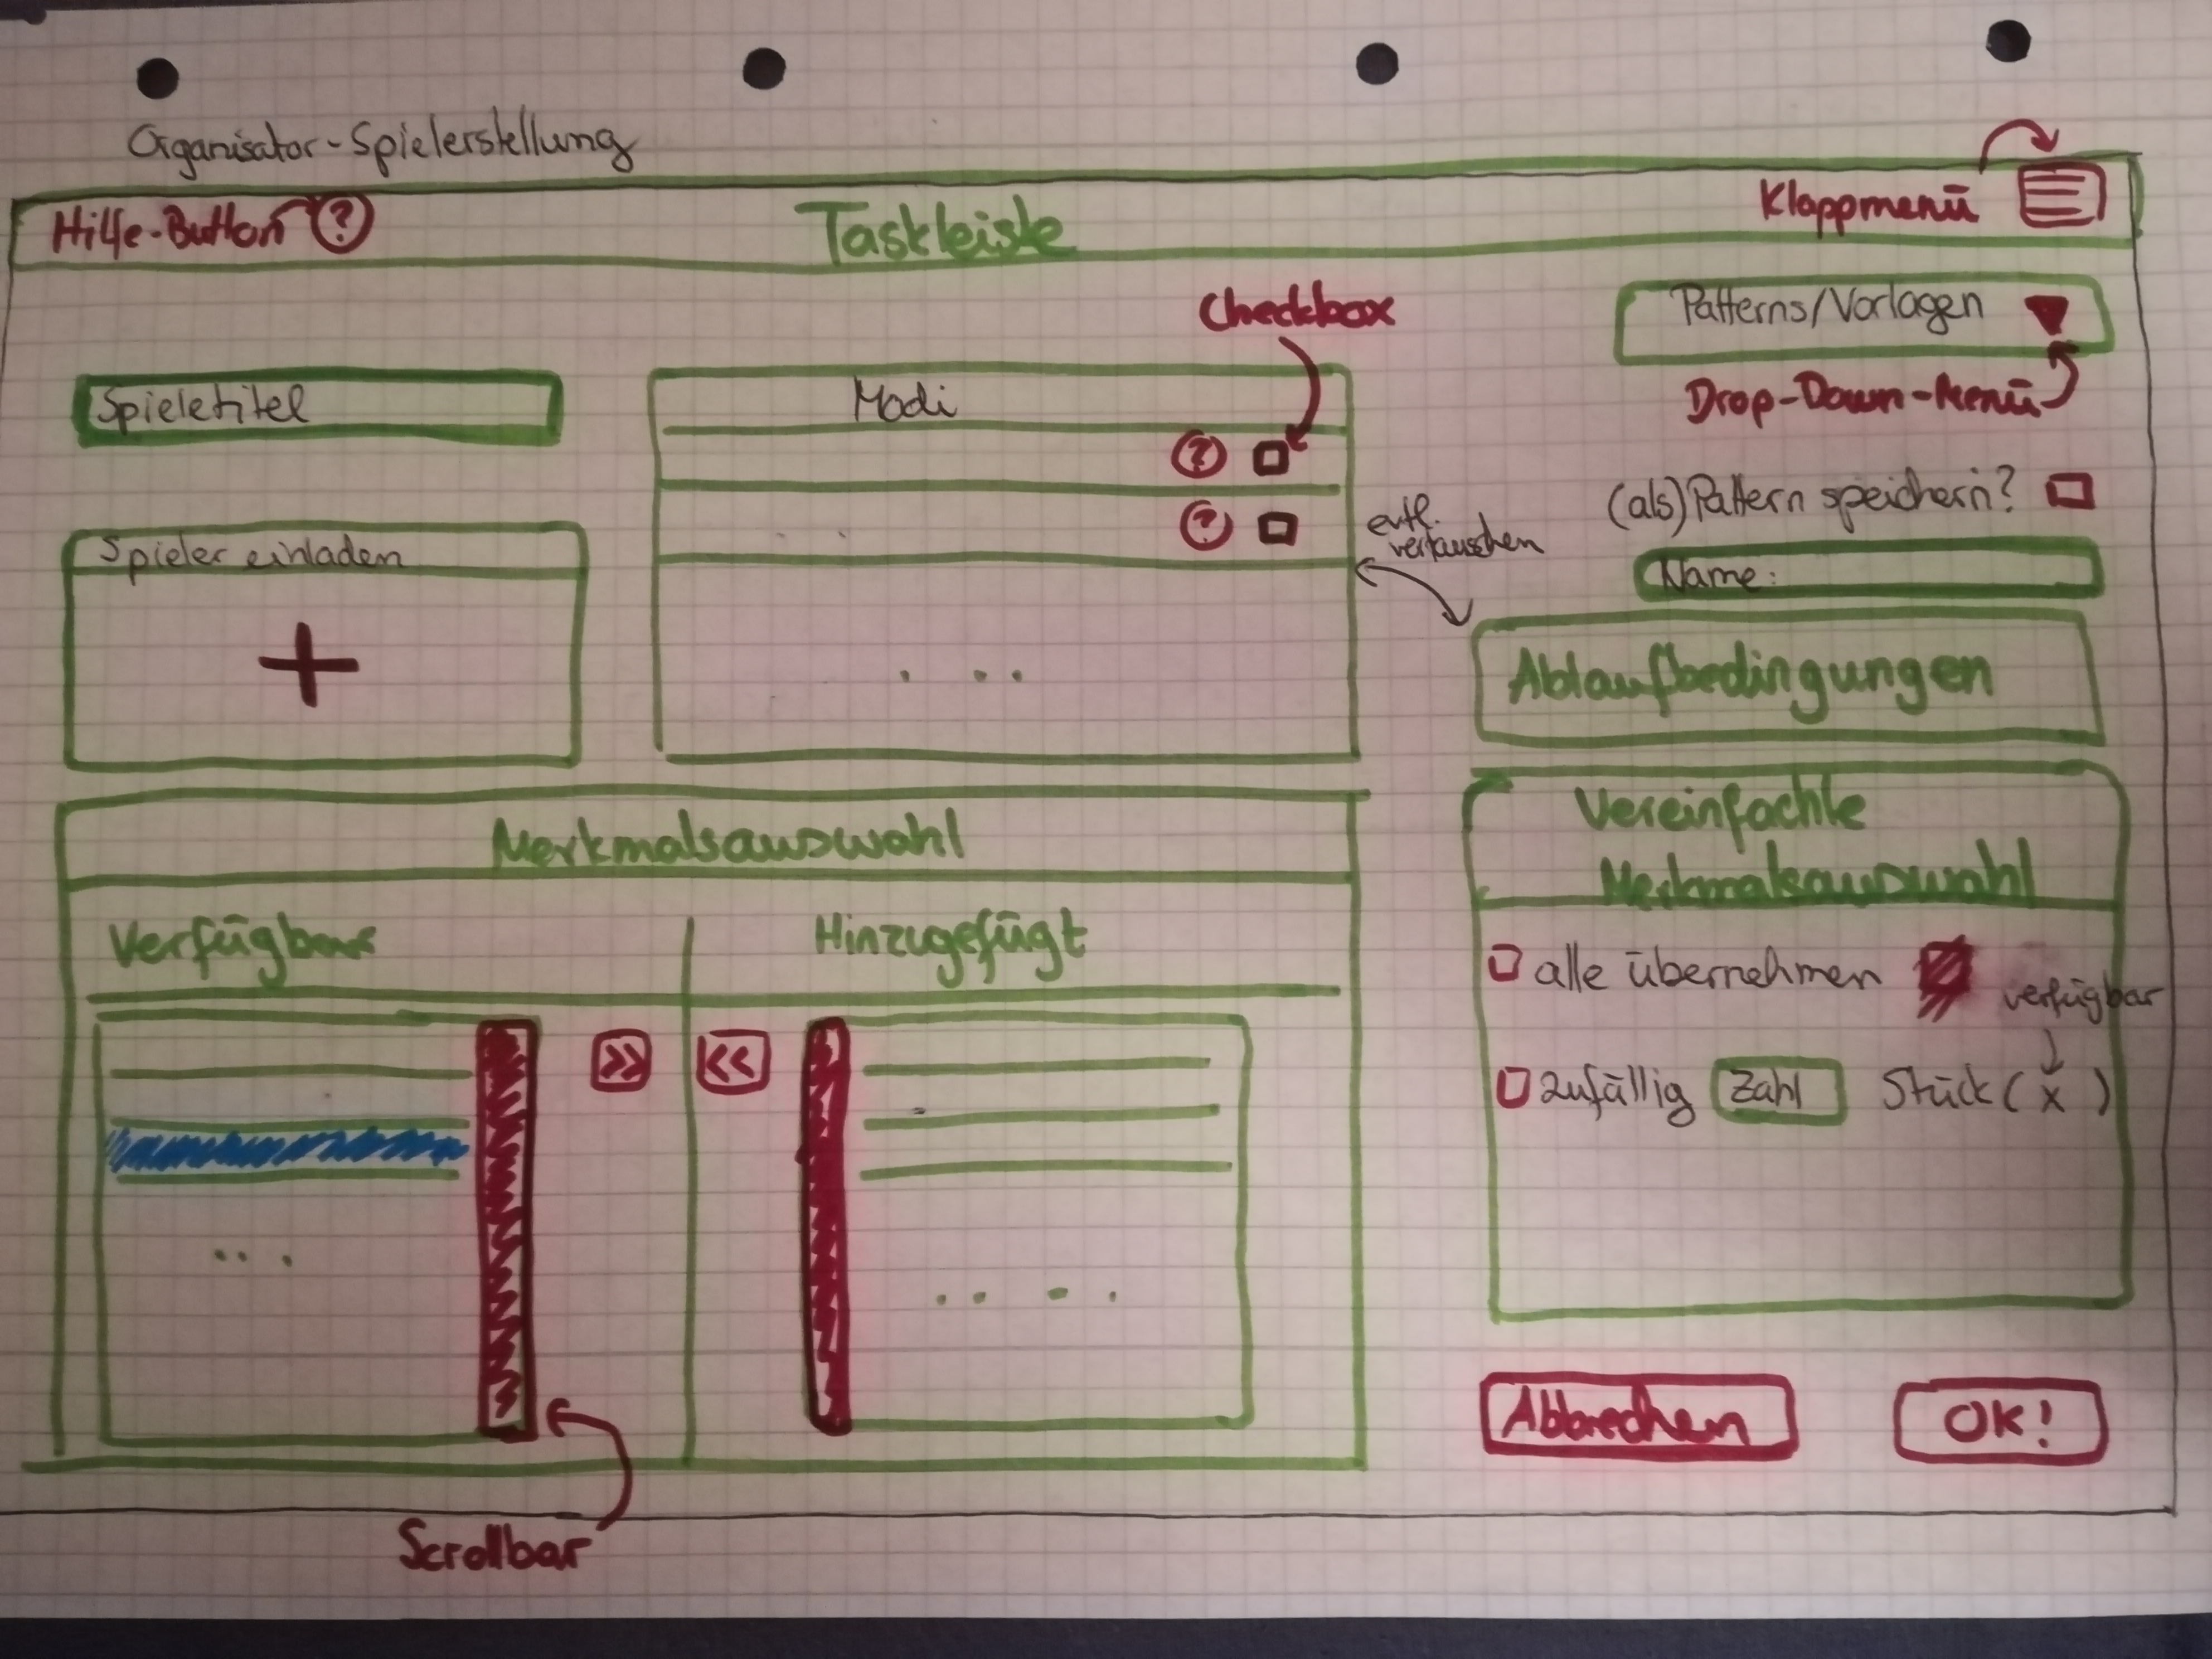
\includegraphics[width=400px]{../pictures/4_Spielerstellung.jpg}

    \subsection{Spieler-Übersicht}
    \label{fig:Spieler-Übersicht}
    \centering
    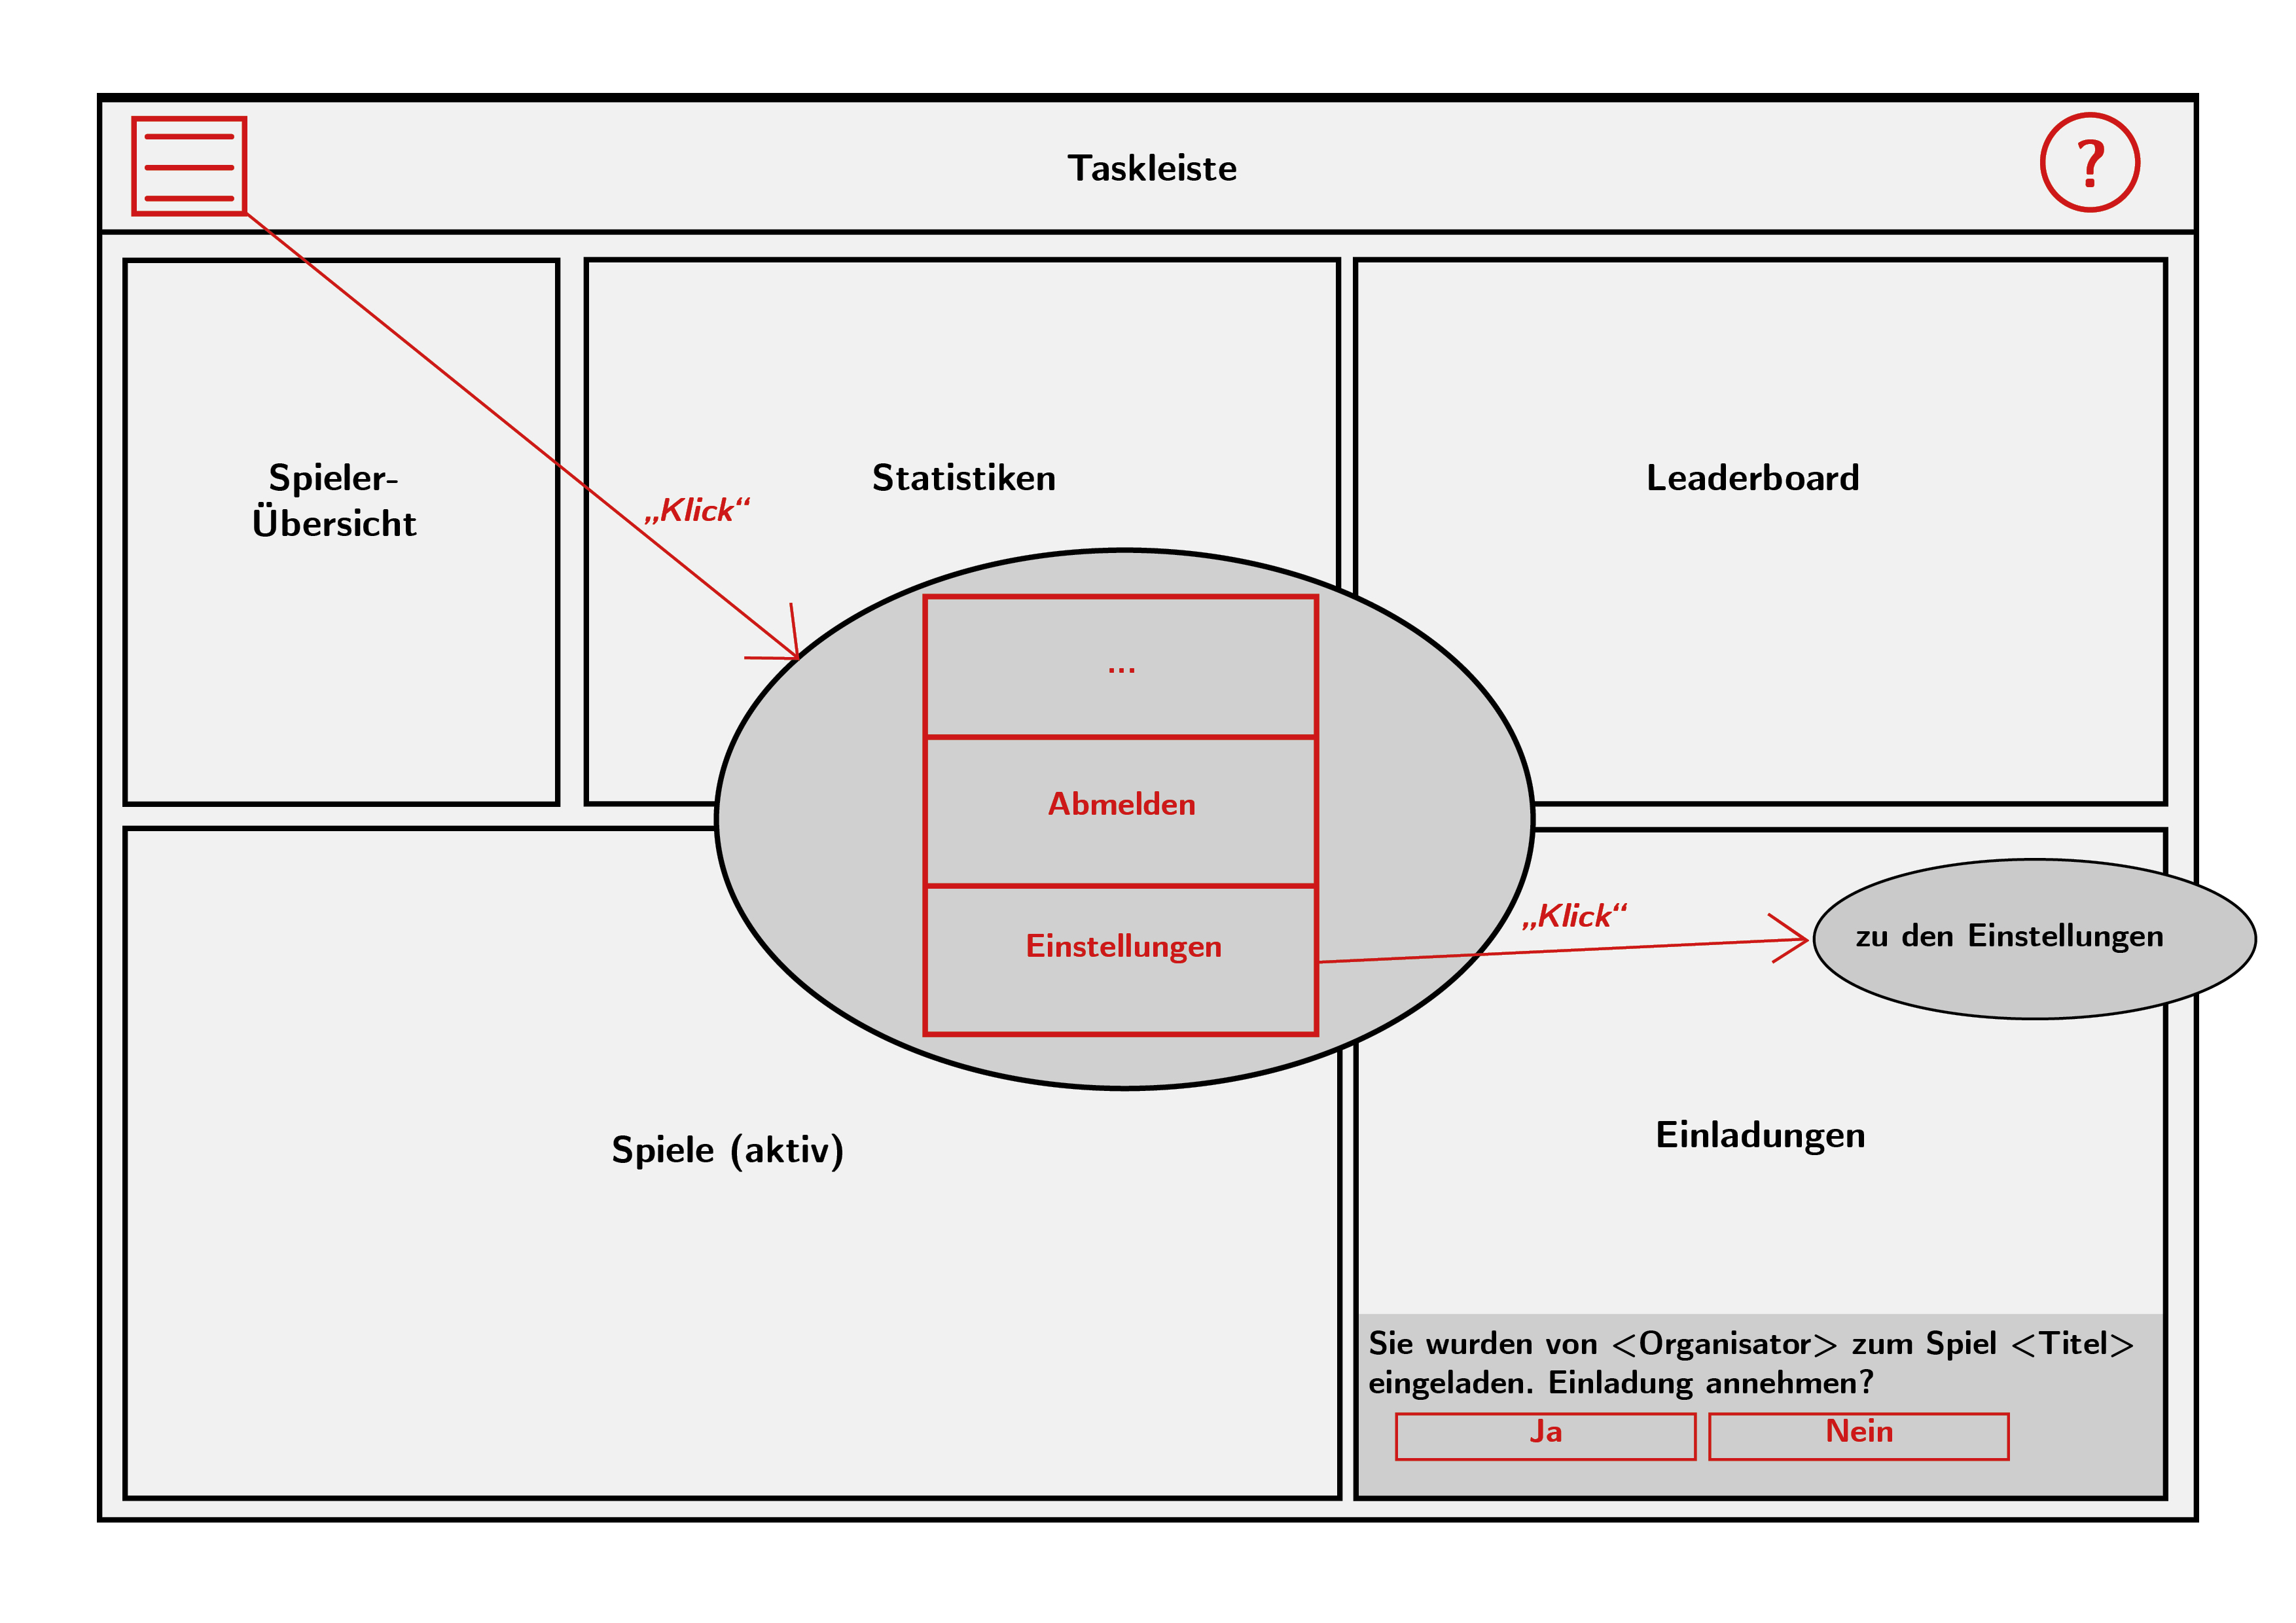
\includegraphics[width=400px]{../pictures/5_Spieler.jpg}

    \subsection{Spiel}
    \centering
    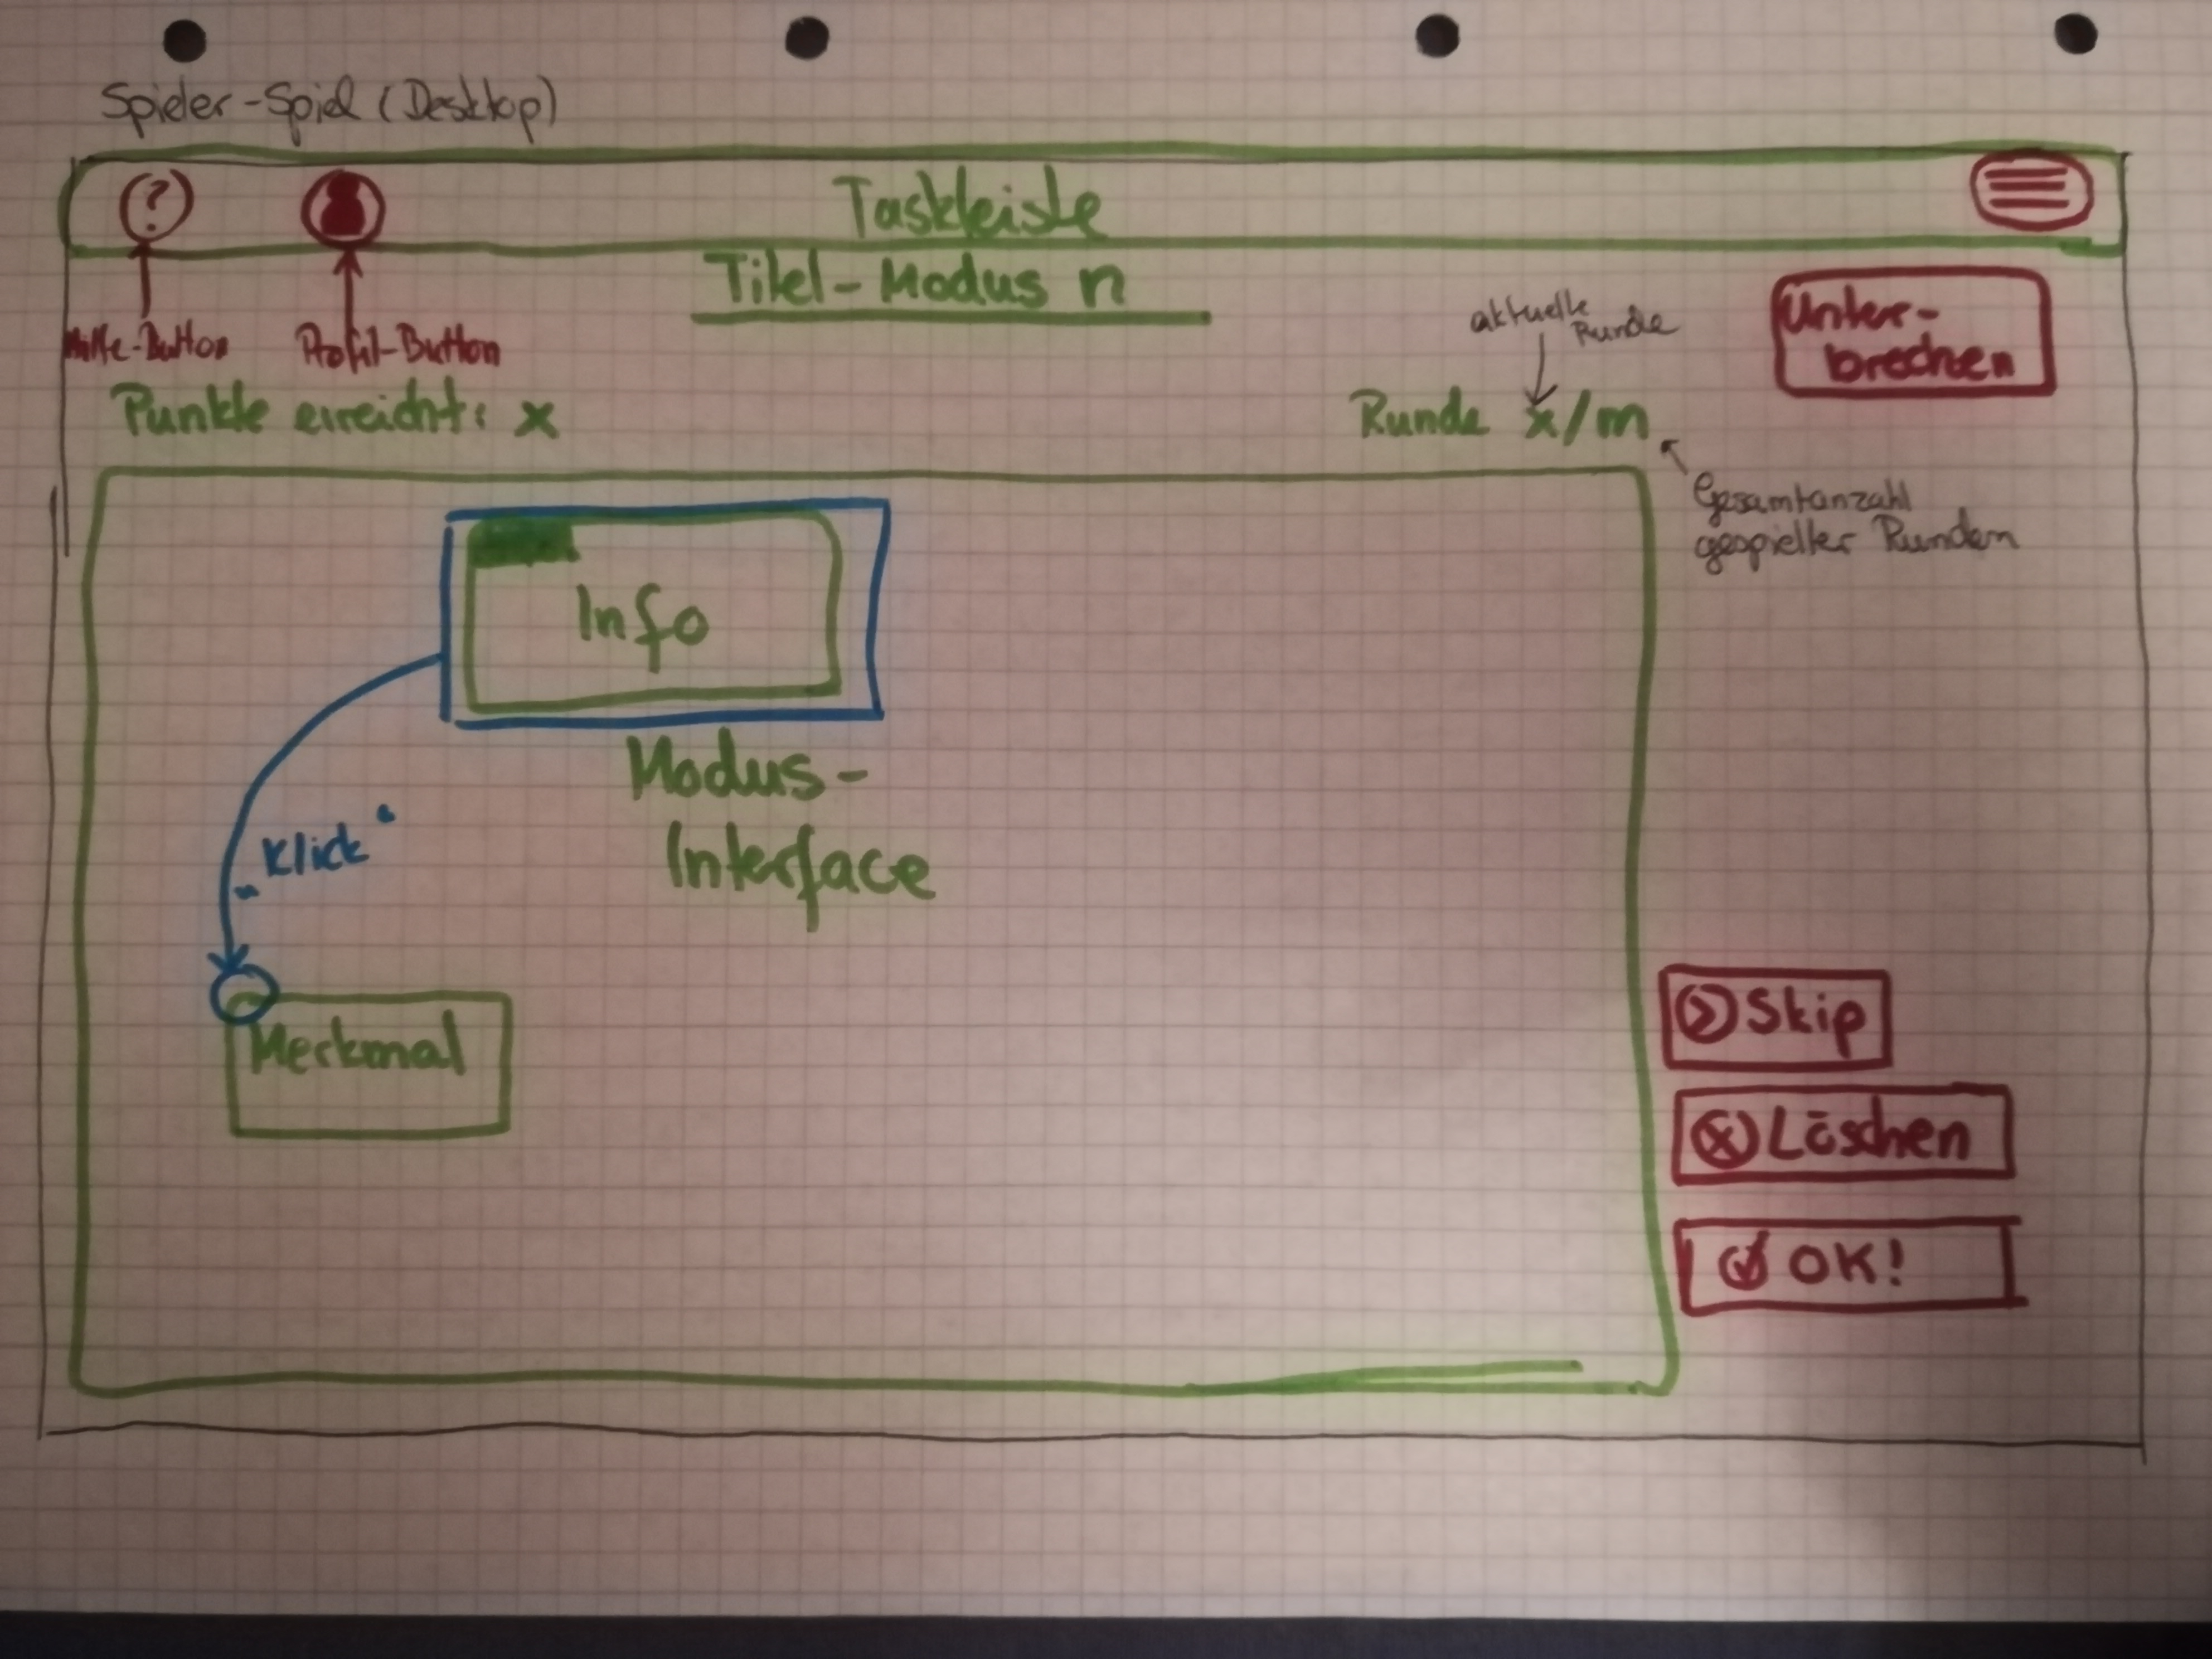
\includegraphics[width=400px]{../pictures/6_Spiel.jpg}

    \clearpage


    \chapter{Glossar}

    \printglossary

\end{document}
